\documentclass{standalone}
\usepackage{pgfplots}


\begin{document}

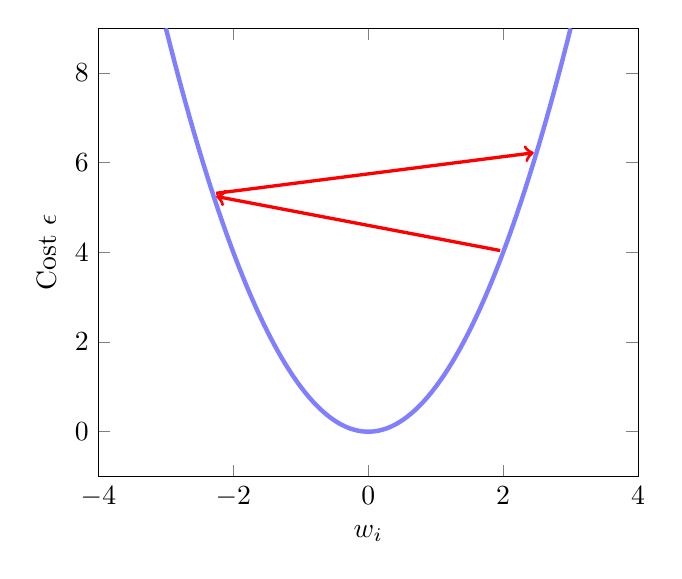
\begin{tikzpicture}
\begin{axis}[xmax=4,xmin=-4,ymax=9, ymin=-1, samples=100, xlabel={$w_i$}, ylabel={Cost $\epsilon$}, title style={font=\huge}]
  % TODO: remove axes

%  \addplot[domain=0:2, red, thick] (x, 2*1*x-1);
%  \addplot[domain=-3:-1, red, thick] (x, 2*-2*x-4);

%  \addplot[domain=0:2, red, thick] (x, 2*1*x-1);
%  \addplot[domain=-3:-1, red, thick] (x, 2*-2*x-4);

%  \addplot[domain=-9:9, gray] (x, 0);
%  \addplot[domain=-9:9, gray] (0, x);
  \addplot[domain=-3:3, blue!50, ultra thick] (x, x*x);

\node (p1) at (axis cs:2.1,4){};
\node (p2) at (axis cs:-2.4,2.3*2.3) {};
\node (p3) at (axis cs:2.6,2.5*2.5) {};
\draw[->, red, very thick](p1)--(p2);
\draw[->, red, very thick](p2)--(p3);


% UNDERSHOOT
%\draw[->, red, very thick] (axis cs:2, 2*2)--(axis cs: 1.76, 1.76*1.76);
%\draw[->, red, very thick] (axis cs:1.8, 1.8*1.8)--(axis cs: 1.56, 1.56*1.56);
%\draw[->, red, very thick] (axis cs:1.6, 1.6*1.6)--(axis cs: 1.41, 1.41*1.41);
%\draw[->, red, very thick] (axis cs:1.45, 1.45*1.45)--(axis cs: 1.25, 1.25*1.26);

% 


% x^2
% find tangent at (1, 1)
% slope of tangent = 2x = 2*1
% intercept of tangent = b = -1

% find tangent at (-2, 4)
% slope of tangent = 2*-2
% intercept = b = -8
% -4*-2 + b = 0

\end{axis}
\end{tikzpicture}

\end{document}